\section{Application existante}

\subsection{Présentation de l'application}
La partie sur laquelle nous travaillons est écrite en C++. Pour des raisons pratiques, le framework 
QtCreator est utilisé, il facilite la création d'applications et d'interfaces graphiques. De même, 
la bibliothèque OpenCV  est largement utilisée dans le projet, elle est open-source et dispose de 
nombreux algorithmes dans le domaine de la vision par oridinateur. Ainsi, le développement de 
l'application est plus rapide car les algorithmes tels que Viola etJones ou Canny sont déjà implémentés.

\subsection{Architecture}
L'application fournie est orientée objet et respecte le principe <<open-close>>. En effet, celle-ci est 
découpée en Business Objects\footnote{Les Business Objects sont des objets métiers qui s'occupent de tâches 
précises}, il est possible de créer et greffer nos propres objets métiers dans l'application. Les Business 
Objects sont hiérarchisés dans une pyramide métier, où les objets métiers en haut de cette pyramide 
sont les plus abstraits et utilisent les resultats de l'étage inférieur. Les objets métiers en bas de 
la pyramide sont les plus proches du flux vidéo brut.\\

\begin{figure}[H]
  \centering
  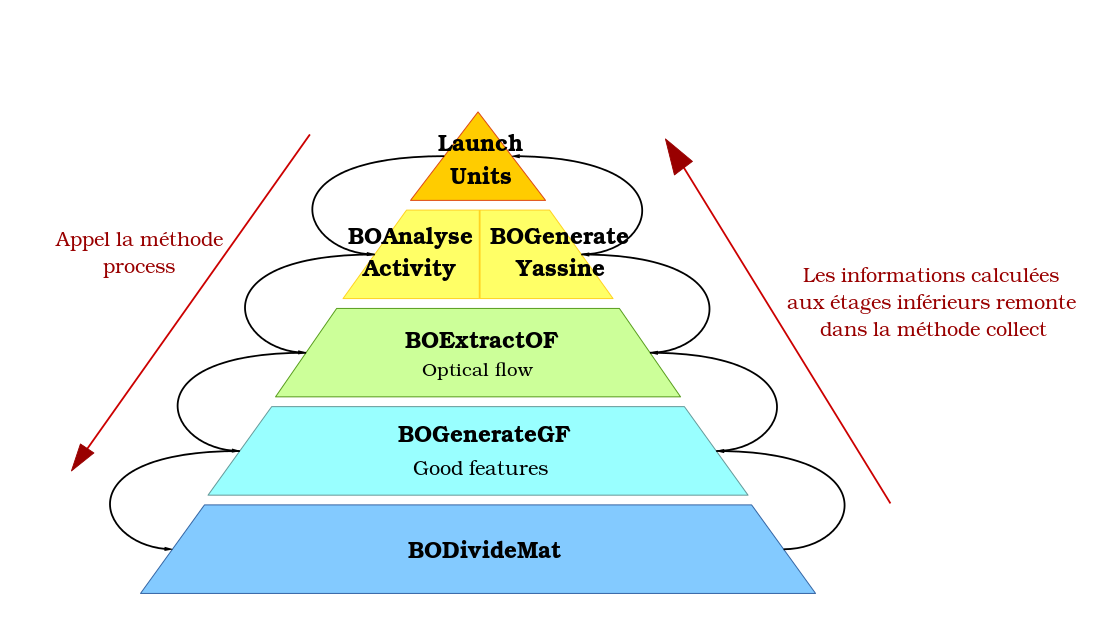
\includegraphics[width=15cm]{image/pyramide.png}
  \caption{Processus d'extraction des informations pyramidales sur le flux vidéo}
\end{figure}
\newpage
Les différentes couches de la pyramide disposent d'une classe métier abstraite. Ces classes 
sont décrites dans la liste suivante :\\

\begin{itemize}
 \item \textbf{BODivideMat} : ces objets métiers découpent une image source en plusieurs images telles que 
 le cadre du visage ou des yeux.
 \item \textbf{BOGenerateGF} : ces objets métiers générent les bonnes particularités (Good Features). 
 À cette étape, le choix des points d'intérêts est effectué, ces points sont dans la zone du visage 
 découpée dans l'étage précédent. Ensuite, les points identiques dans l'image précédente et l'image 
 courante sont conservés.
 \item \textbf{BOExtractOF} : ces objets métiers extraient les flux optiques (Optical Flows) à partir 
 des points générés lors de l'étape précédente. Les flux optiques représentent les mouvements à l'intérieur 
 du visage et doivent être invariants aux mouvements du visage, de la personne ou de la caméra.
 \item \textbf{BOAnalyseActivity et BOGeneteYassine} : ces objets métiers analysent les résultats 
 des flux optiques afin de déterminer les informations sur l'activité à l'intérieur du visage.
 \item \textbf{Lauch Units} : cette unitée n'est pas un objet métier, elle crée les objets métiers des 
 couches inférieures afin d'avoir une exécution du programme qui utilise ces Business Objects.
\end{itemize}
\ \\

Pour notre projet, nous travaillons dans la couche basse de la pyramide. Cette couche divise
les images du flux vidéo en diverses régions d'intérêt telles que la région du visage, puis 
des yeux.

% fusion
\subsection{Détection du visage et des yeux}

L'application est divisée en deux parties. La première recherche le visage grâce à
l'algorithme de Viola et Jones, et la seconde recherche les yeux dans la région délimitée
précédemment.

\subsubsection{Détection du visage}
L'algorithme de Viola et Jones\cite{Viola04robustreal-time} est une méthode qui a été créée pour la détection de visages dans une 
image. Cette méthode s'est par la suite généralisée à toutes sortes d'objets. L'algorithme nécessite une 
base de connaissances composée des caractéristiques de l'objet recherché. Elle est utilisée dans un 
apprentissage supervisé, c'est à dire que l'algorithme a besoin de données représentant
l'objet à détecter pour classifier les caractéristiques de celui-ci.\\

Cet algorithme est basé sur des caractéristiques pseudo-Haar qui crée des masques rectangulaires et adjacents
dans différentes zones de l'image. Chaque masque calcule l'intensité des pixels qu'il contient, puis l'algorithme fait
la différence entre les masques blancs et les masque noirs. Cette méthode va permettre de détecter des contours ou des changements de 
texture.\\

\begin{figure}[H]
\center

\includegraphics[width=5cm]{image/pseudo_haar.png}
\caption{Exemple de caractéristiques pseudo-Haar utilisé pour l'algorithme Viola et Jones}
\end{figure}

Pour améliorer les perfomances de leur algorithme, Viola et Jones utilisent la méthode Adaboost. Son
principe est de séléctionner les caractéristiques les plus performantes pour la détection de l'objet grâce à
un calcul de probabilité utilisant l'entropie\footnote{valeur mesurant l'incertitude d'une donnée} des données.\\

Cet algorithme est très efficace pour la détection de visage de l'application, mais nous ne pouvons le mettre
en oeuvre pour la détection des yeux faute de temps. De plus, la base de connaissances nécessaires pour cet 
algorithme doit posséder des miliers d'exemples qu'il nous est impossible de rassembler. C'est pourquoi
un autre algorithme a été utilisé pour la détection des yeux.

\subsubsection{Détection des yeux}
Une fois que la région du visage est reconnue dans le flux vidéo, nous cherchons à détecter les yeux. 
L'algorithme de détection des yeux déjà existant dans l'application permet une détection des yeux 
robuste, mais assez peu précise. Cet algorithme se déroule en plusieurs étapes. D'abord, la région du visage 
retrouvé par la méthode de Viola et Jones est égalisée. Ensuite, elle est scannée de bas en haut afin de
trouver les yeux avant les sourcils. Dans un même temps l'algorithme essaie de retrouver les yeux via la
méthode Means Shift\footnote{technique d'analyse permettant de trouver les maxima dans une fonction de densité}.



